\XeTeXlinebreaklocale "zh"
\XeTeXlinebreakskip = 0pt plus 1pt

\documentclass[11pt,a4paper]{article}

\usepackage{colortbl}
\usepackage{minted}
\usepackage{xltxtra,fontspec,xunicode}
\usepackage[hidelinks]{hyperref}

\usepackage{graphicx}
\usepackage{float}

\defaultfontfeatures{Mapping=tex-text,Scale=MatchLowercase}
\setmainfont{DejaVu Serif}
\setsansfont{DejaVu Sans}
\setmonofont{DejaVu Sans Mono}
\usepackage[slantfont,boldfont]{xeCJK} % 允许斜体和粗体
\setCJKmainfont{WenQuanYi Zen Hei}
\setCJKsansfont{WenQuanYi Zen Hei}
\setCJKmonofont{WenQuanYi Zen Hei Mono}

\title{Rule-Based Regular Routing Method}
\author{
	周聿浩\\ \texttt{2016011347} \and
	翁家翌\\ \texttt{2016011446}
}

%\setlength{\parindent}{2em}
%\setlength{\parskip}{0.5em}

\begin{document}
\maketitle
\tableofcontents
\section{介绍}
\qquad
在一个电路板上,给定一个均匀分布的$n\times n$个内部节点,要求确定电路板的大小,计算各个节点到电路板边界的路径,使得各个路径不相交并且长度之和最短。

为了解决这个问题,本项目实现了基于费用流的布线方案,该方案能够获得最优解,然而由于不适应与大规模的数据,因此又实现了基于规则的布线方案,该方案可以在可以接受的时间内得到较优的解。关于具体的实现算法见第 \ref{algo} 节,具体的设计思路见第 \ref{sys-arch} 节。

我们支持将计算得到的方案以图片形式输出到文件或窗口,同时也支持以原始路径的形式保存到文件。并且支持从文件中读取原始数据并且显示到窗口。

目前为止,我们基于规则的算法最大支持$150\times 150$个节点。

\begin{figure}[htpb]
	\centering
	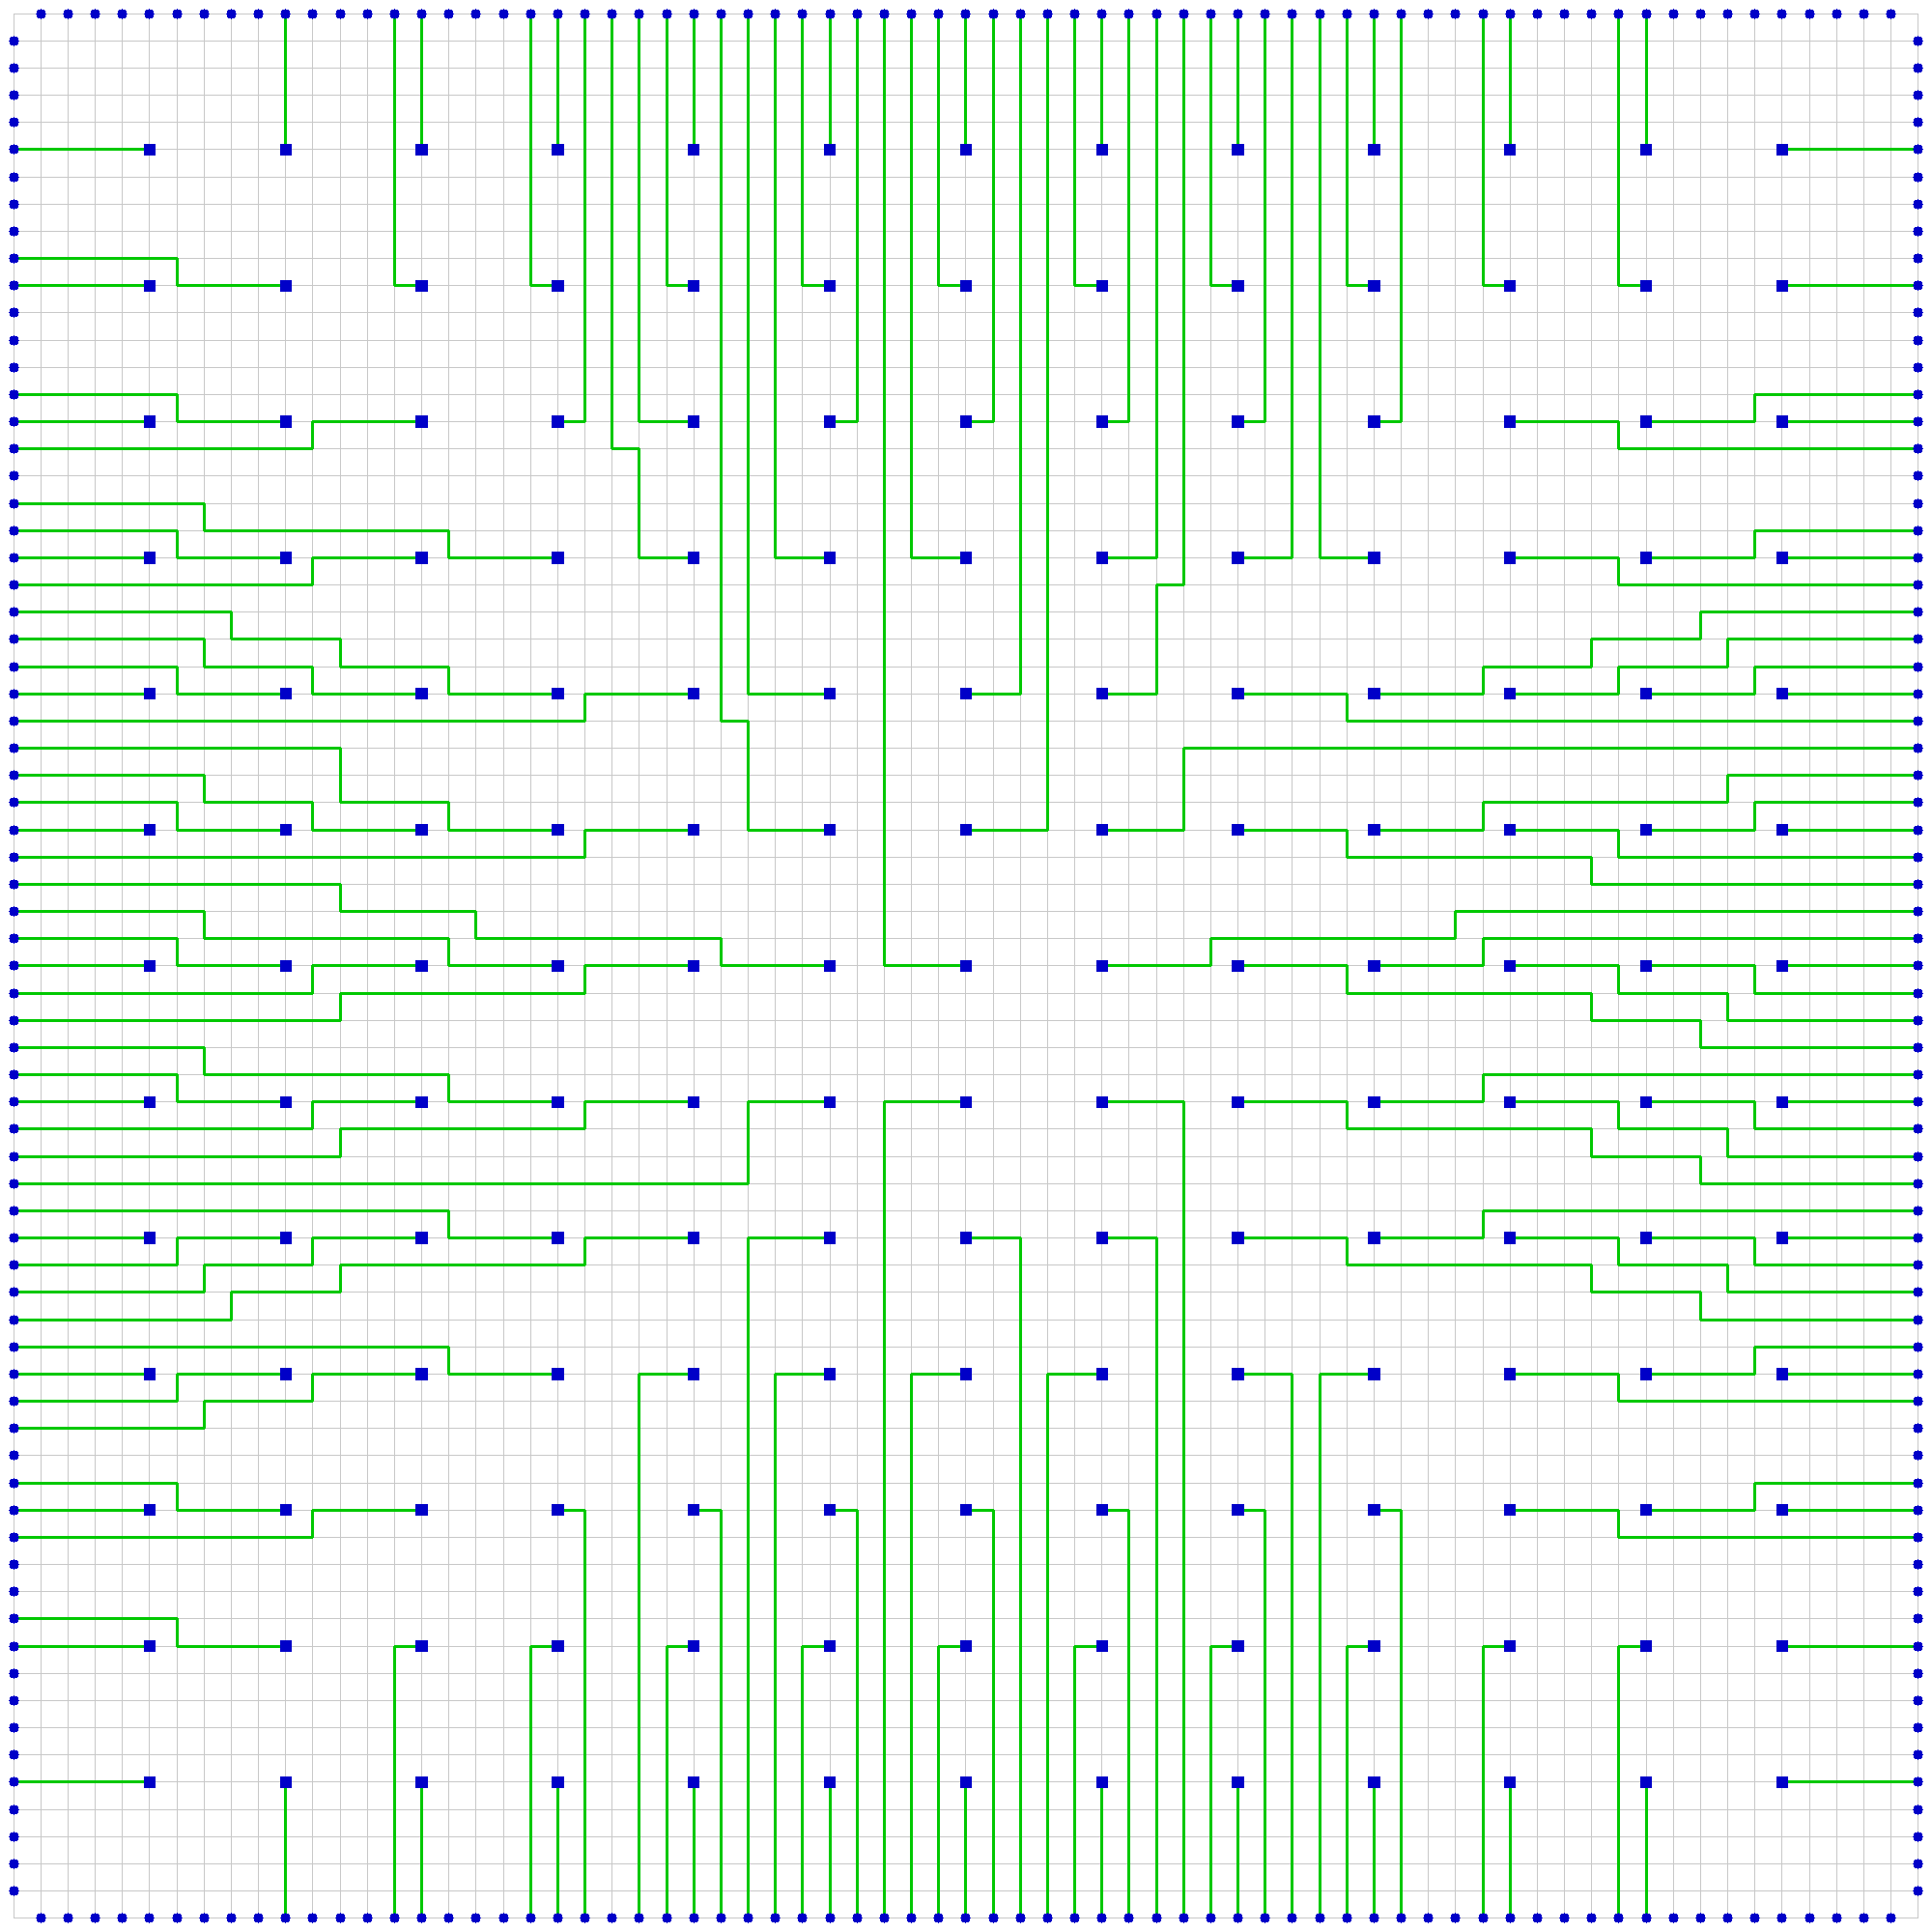
\includegraphics[height=2in]{../testcase/small-cases/13x13-71x71.png}
	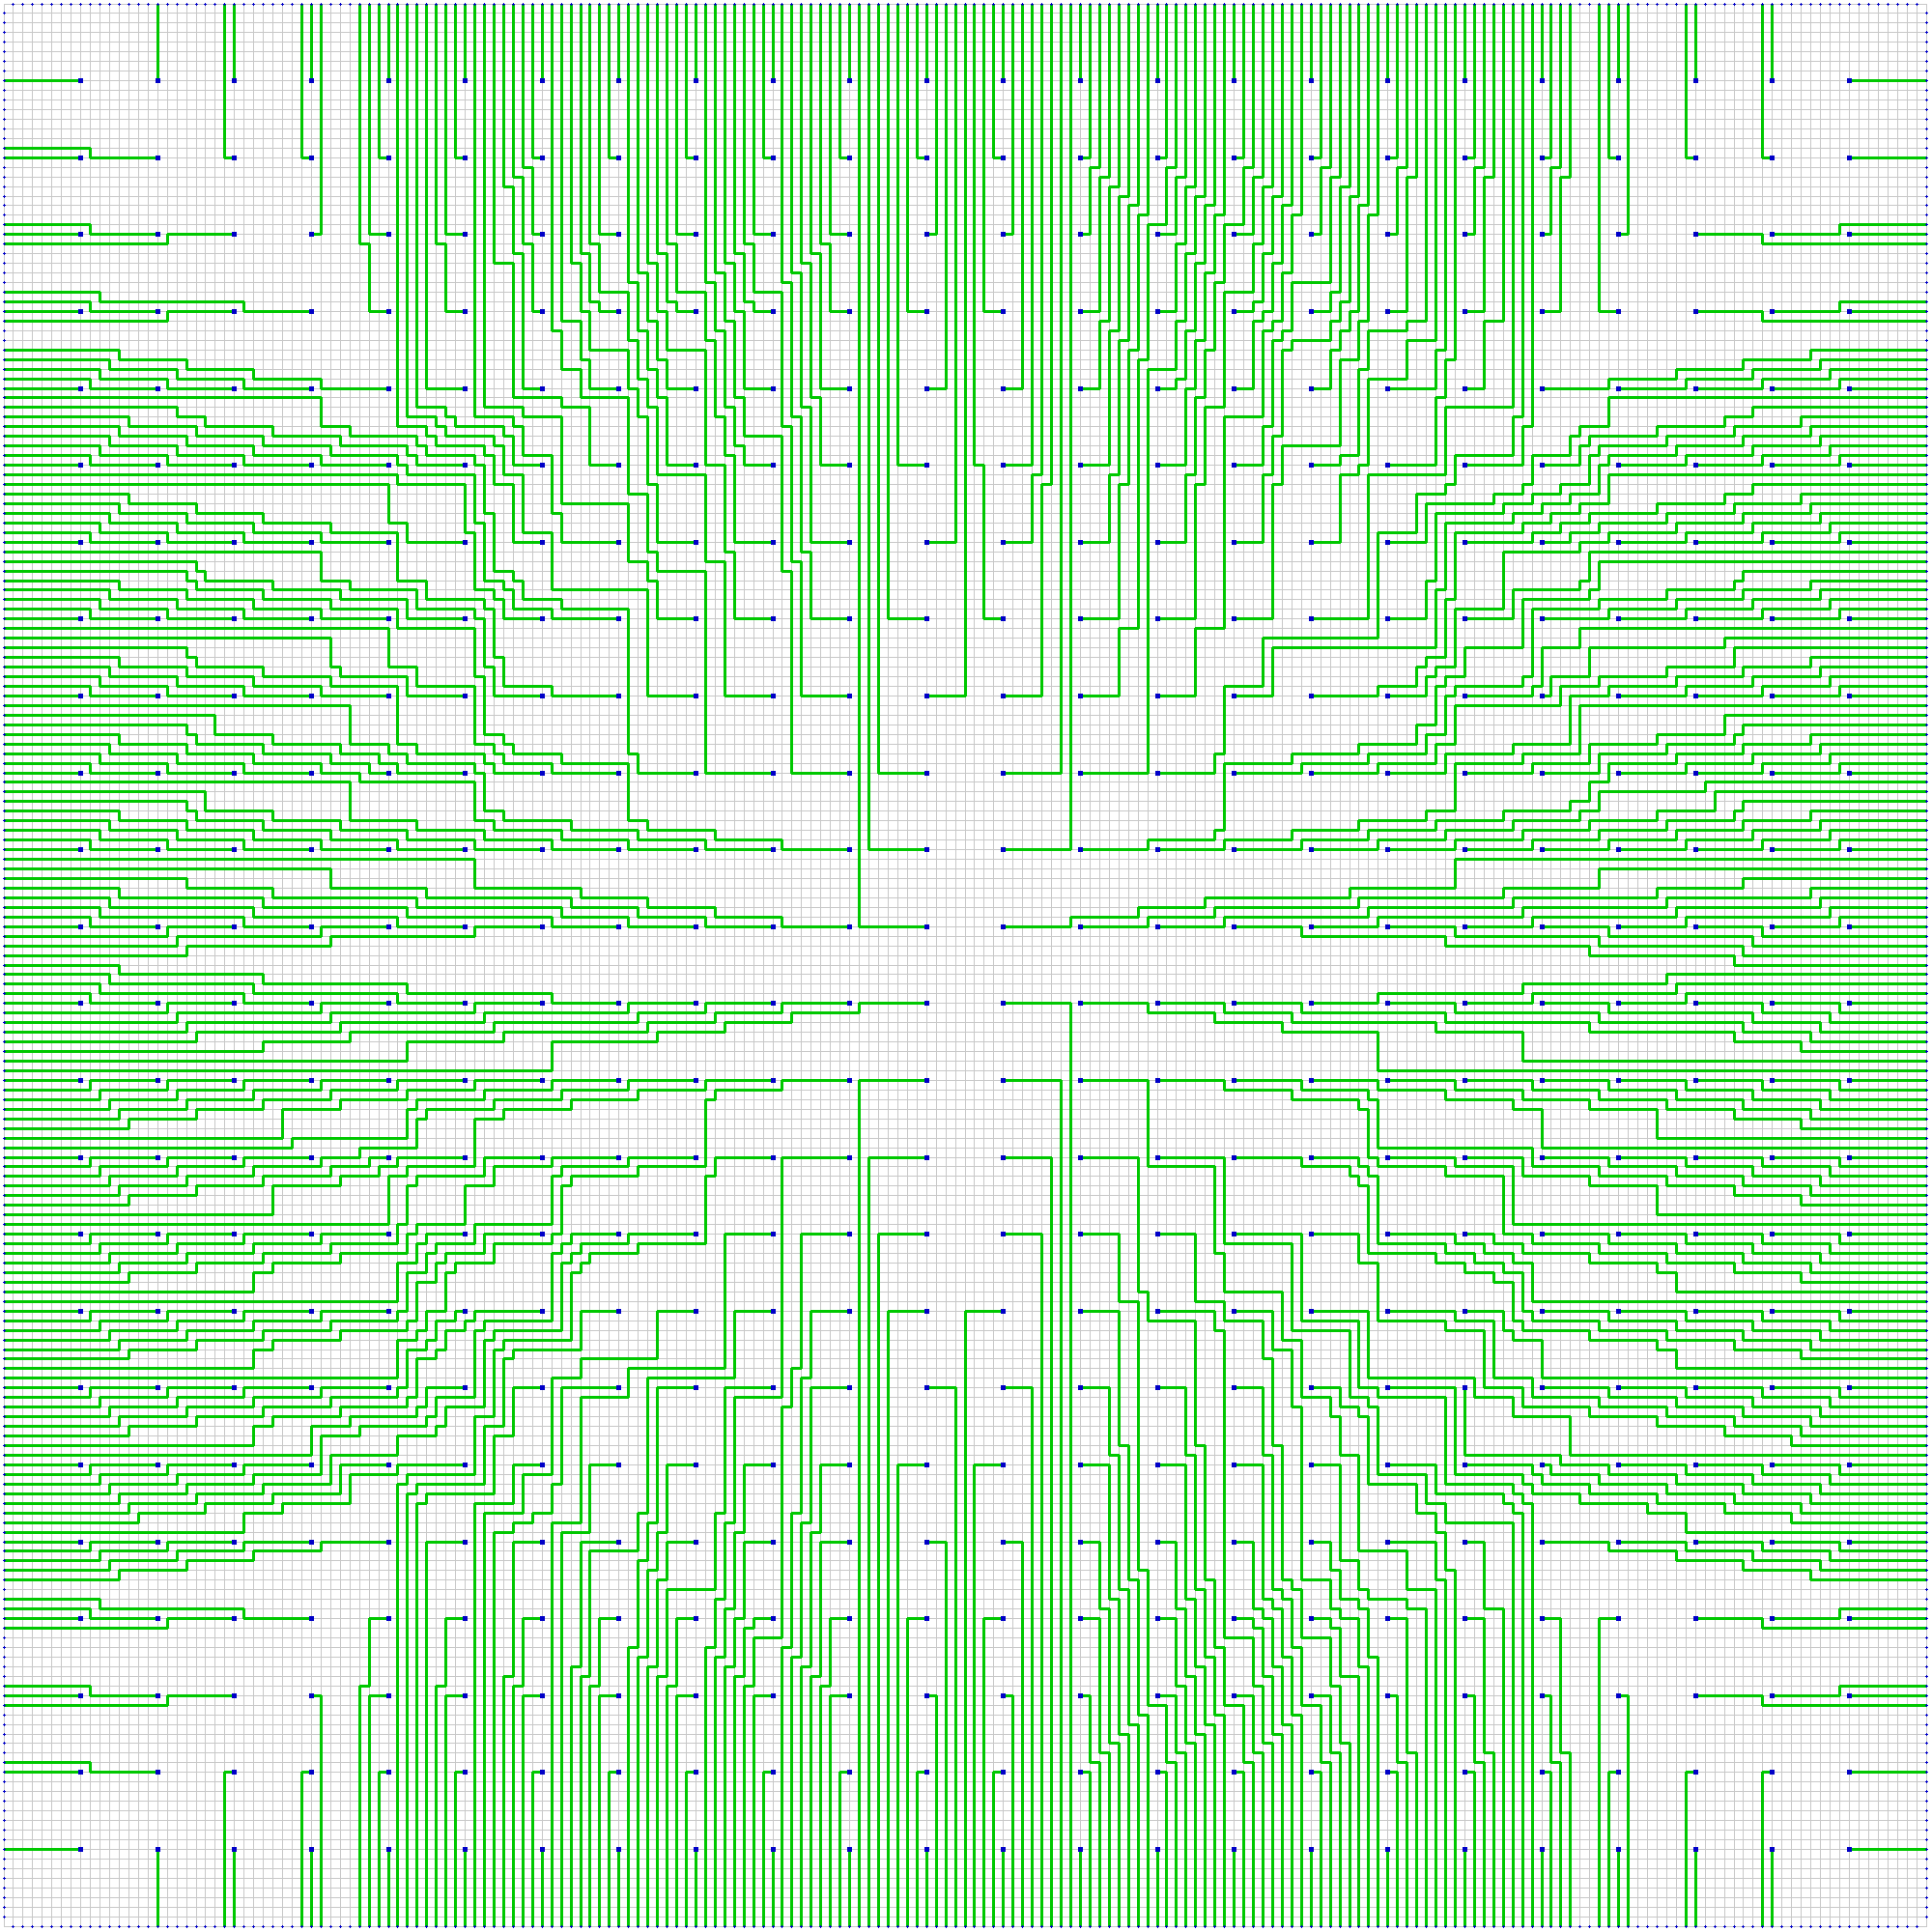
\includegraphics[height=2in]{../testcase/small-cases/24x24-201x201.png}
	\caption{两个基于网络流方案的例子}
\end{figure}

\section{使用方法}
\subsection{编译及运行}
	\qquad
	本项目依赖一些第三方库:
	\begin{itemize}
		\item Boost
		\item OpenCV
	\end{itemize}

	并且使用 CMake 来进行 Makefile 的生成,可以在进入 src 目录后运行如下代码进行编译
	\begin{minted}{bash}
    mkdir build
    cd build
    cmake ../
    make
	\end{minted}

	编译完成后使用 \mintinline{bash}{./main} 来运行程序,或可以使用 \mintinline{bash}{./main --help} 来查看帮助。

	如果你想用基于网络流的算法计算节点大小为18x18的布线方案,可以运行如下

	\begin{minted}{bash}
    ./main -n 18 -a flow
	\end{minted}

	如果你想保存路径信息,并且不想显示窗口,则可以运行如下

	\begin{minted}{bash}
    ./main -n 18 -p 18x18.data --no-window
	\end{minted}

	如果你想将结果保存为大小为3000x3000的图片,并在窗口以700x700的大小显示,则可以运行如下

	\begin{minted}{bash}
    ./main -n 18 --img-size 3000 --win-size 700
	\end{minted}

	如果想要查看具体的计算过程,则可以运行如下

	\begin{minted}{bash}
    ./main -n 30 --show-step -d 500
	\end{minted}
\subsection{具体参数}
	\begin{itemize}
	\item[-h] 查看帮助。
	\item[-n] 指定x方向以及y方向有多少个节点,默认为12。
	\item[-a] 指定算法,有基于规则(rule)和基于网络流(flow)两个方法,默认为 rule。
	\item[-p] 将结果存储到指定文件(若没有这个参数则不存储)。
	\item[-i] 从指定文件读入结果并且显示。
	\item[-o] 将结果以图片形式存储到文件。
	\item[-{}-img-size] 指定存储的图片大小,默认为2000px。
	\item[-{}-win-size] 指定显示的窗口大小,默认为800px。
	\item[-{}-no-window] 不在窗口显示结果。
	\item[-{}-show-step] 显示计算的具体步骤。
	\item[-d] 指定两个计算步骤的显示间隔时间(单位为ms,默认为1)。
	\end{itemize}


\section{系统结构} \label{sys-arch}
\qquad 
在 src 中主要有这样几个文件:

\begin{itemize}
\item {\bf main.cpp} 主要实现了和用户交互的逻辑
\item {\bf vertex.h} 主要实现了基本的节点类型 Vertex
\item {\bf path.h/cpp} 主要实现了基本的路径类型 Path
\item {\bf route.h/cpp} 整个路径规划算法的抽象接口 Route,同时定义了一些辅助函数用于输出等。下面三个是这个抽象类的具体实现:
	\begin{itemize}
	\item {\bf route\_network\_flow.h/cpp} 基于网络流的布线方法具体实现
	\item {\bf route\_rule\_based.h/cpp} 基于规则的布线方法的具体实现
	\item {\bf route\_input\_adapter.h/cpp} 用于读取存储于文件中的路径信息的适配器
	\end{itemize}
\item {\bf visualization.h/cpp} 用于可视化算法输出
\end{itemize}

Route 的具体实现都不对用户可见,利用一个委托函数来创建其实例同时转换为基类的指针。为了减少用户手动删除造成的不必要错误,使用 std::shared\_ptr 来管理内存。具体实现大致如下:

\begin{minted}{c++}
namespace {
    class RouteNetworkFlowImpl : public Route
    {
    public:
        void compute() {
            // implementation
        }
    };
} // unnamed namespace

RoutePtr get_network_flow_algo()
{
    return std::make_shared<RouteNetworkFlowImpl>();
}
\end{minted}


\section{算法介绍} \label{algo}
\subsection{基于网络流的布线方案}
\qquad
首先分析可以知道,题目可以抽象为给定一张图,寻找一些点不相交路径,使得总长度最短。

现在对于棋盘中的每个节点$u$,由于只能经过一次,将其拆成两个节点$u_{in}, u_{out}$,分别表示进入这个节点的边和从这个节点出去的边。连接一条费用为$0$,流量为$1$的边$(u_{in}, u_{out})$来表示节点只能经过一次的这个限制。

另外对于每一个节点,由于可以向其相邻节点前进,因此对于每一对相邻的节点$(u, v)$,连接一条费用为$1$,流量为$1$的从$(u_{out}, v_{in})$的边。

此外对于每一个内部节点$u$,从源$s$向$u_{in}$连接一条费用为$0$,流量为$1$的边,对于每一个边界节点$v$,从$v_{out}$向汇$t$连接一条费用为$0$,流量为$1$的边。

这样,计算最小费用最大流之后就可以得到最优方案了。

此外还有一个关于最小电路板大小的问题,可以利用二分答案来进行计算。即每次判断这个网络是否满流,而这个计算过程中只需要判断合法性而无需最优性,我们可以利用最大流算法而忽略费用以提高速度。
\subsection{基于规则的布线方案}
\qquad
该方法的所有源代码均在route\_rule\_based.h和route\_rule\_based.cpp中。整体的思路是将整个正方形区域划分成四个小块分别对其进行处理,最后将其合并成一整张图。就像这样:

\begin{figure}[H]
	\centering
	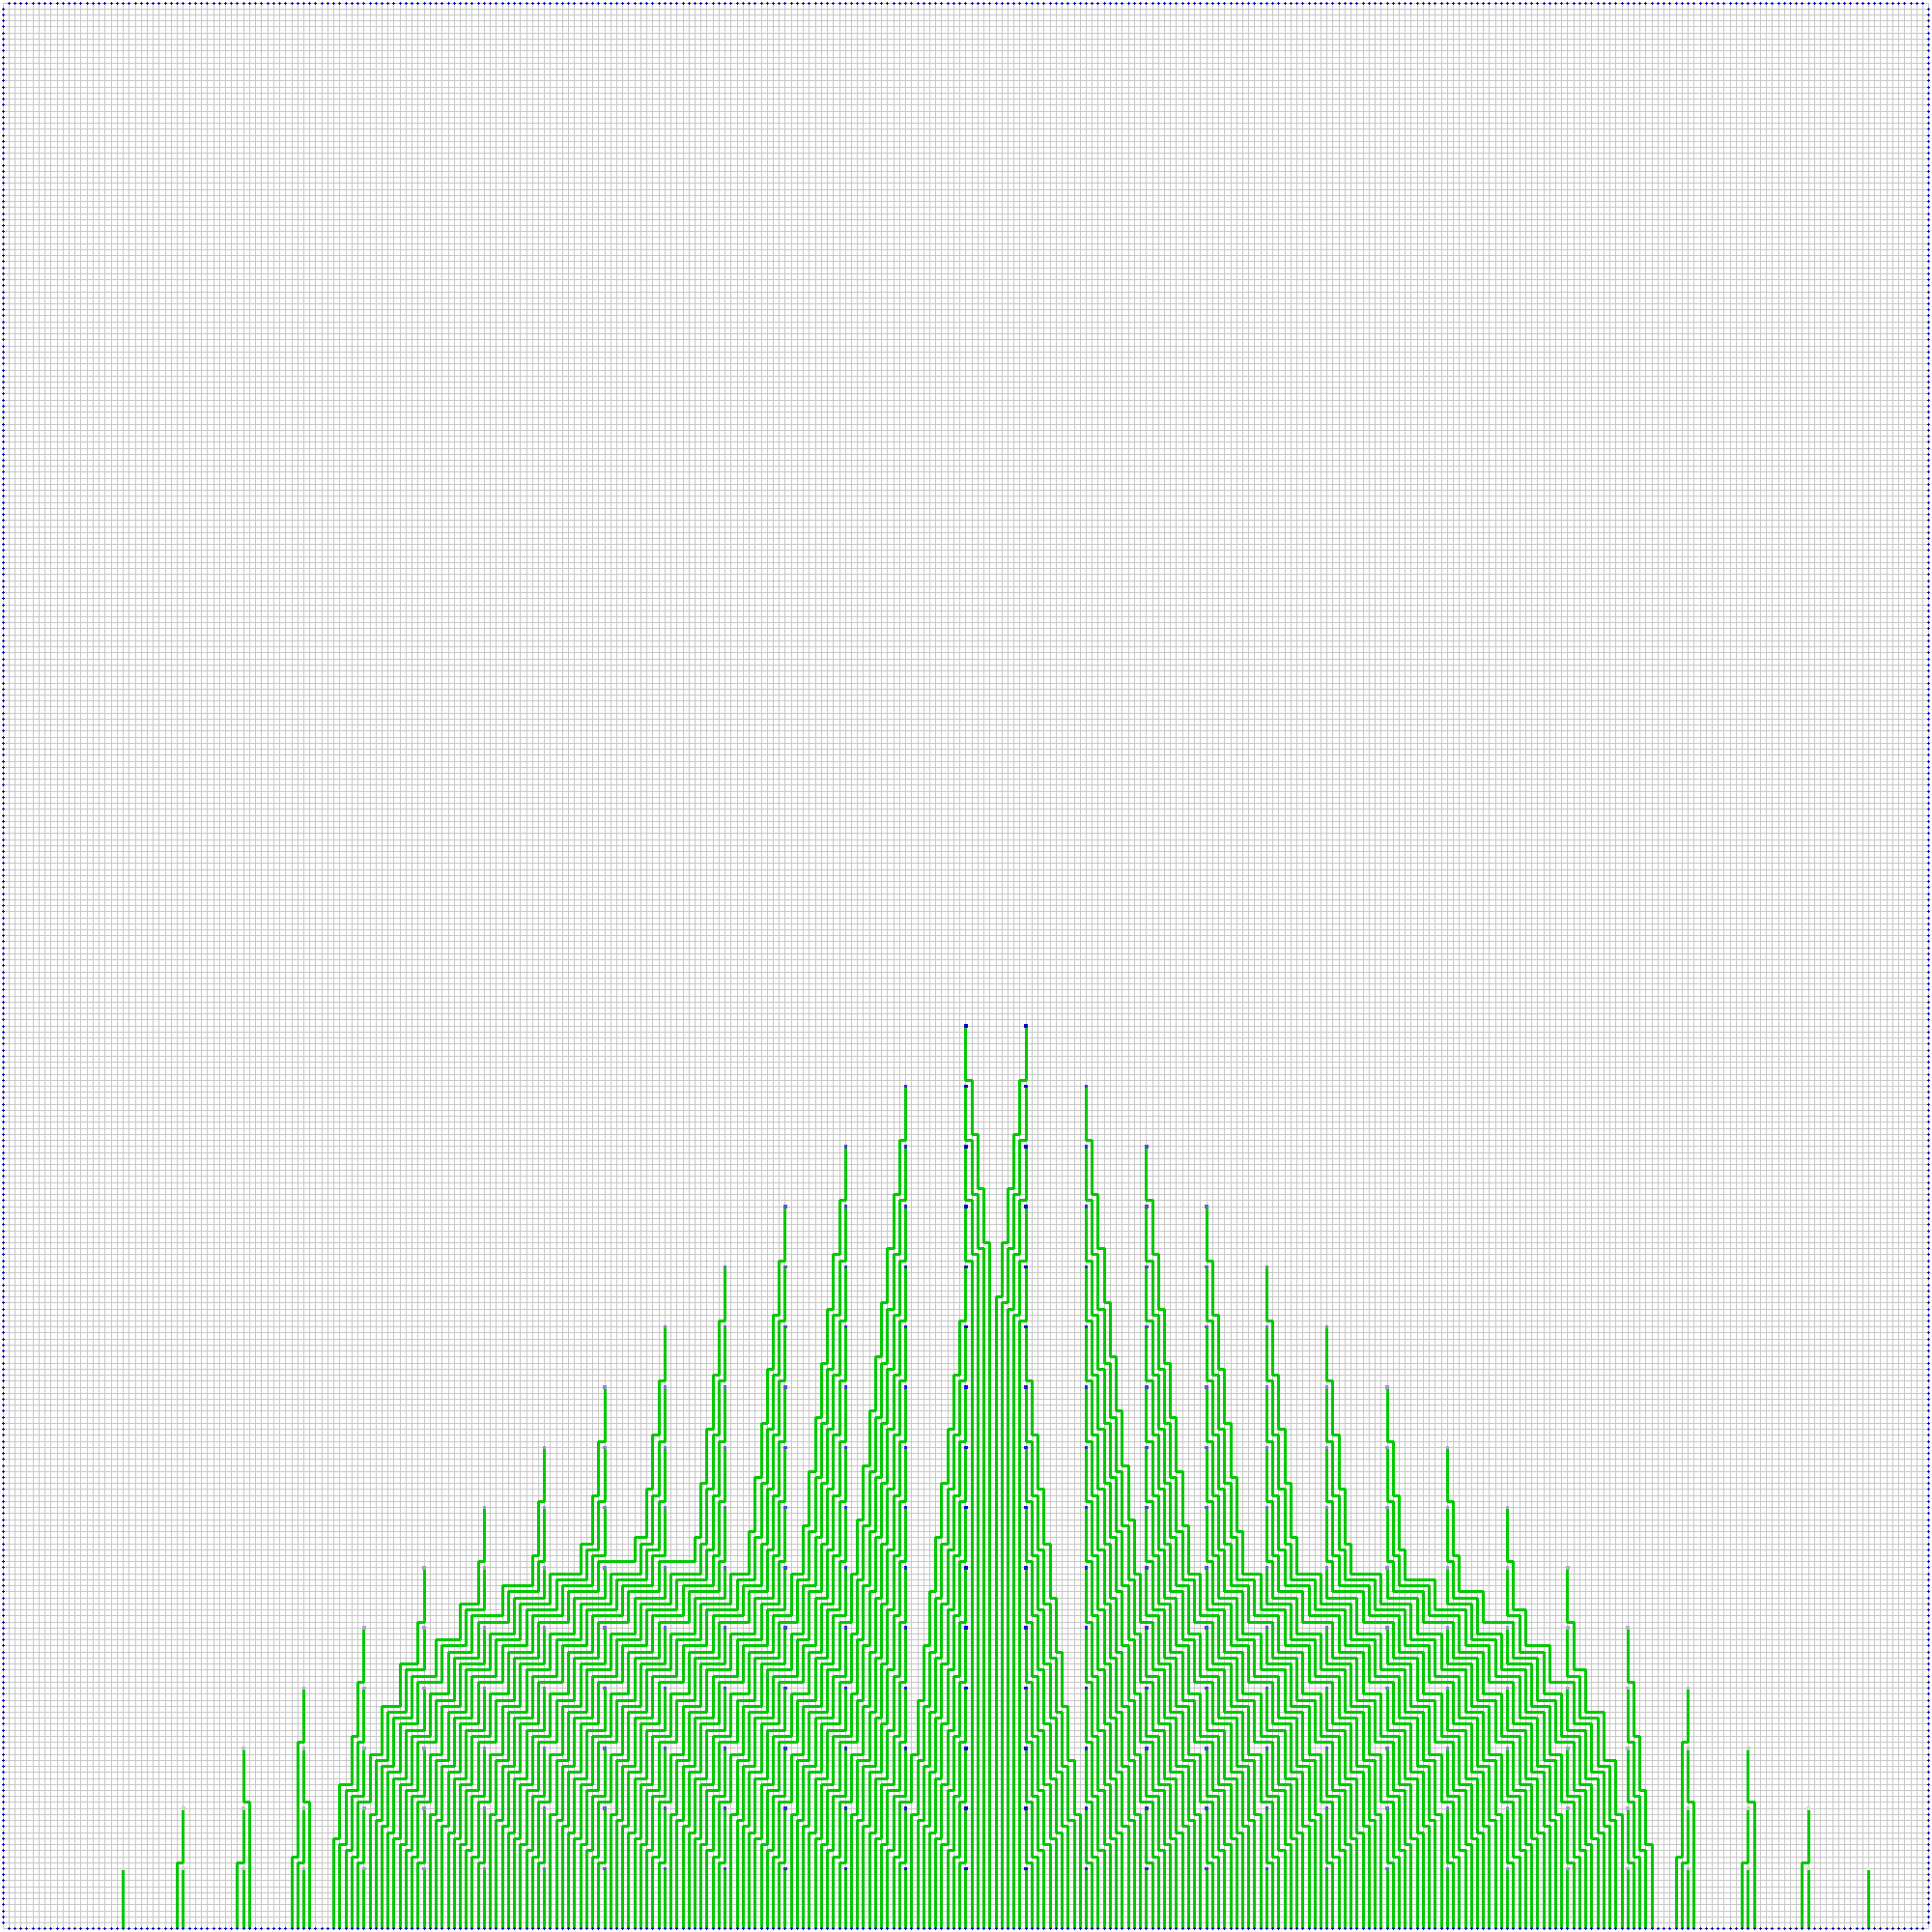
\includegraphics[width=2in]{31.png}
\end{figure}

下半部的三角形会如法炮制地在左部、右部和上部生成,从而构成结果。

\subsubsection{算法设计}
\qquad
\begin{enumerate}
	\item 将正方形点集划分为四个三角形区域,尽量保证均匀划分。以下只考虑在一个三角形内部的情况。
	\item 将最外侧的点直接连出去。由于间隔数的限制,可以证明这些点在最优解下一定只有如下方案。
	\begin{figure}[H]
		\centering
		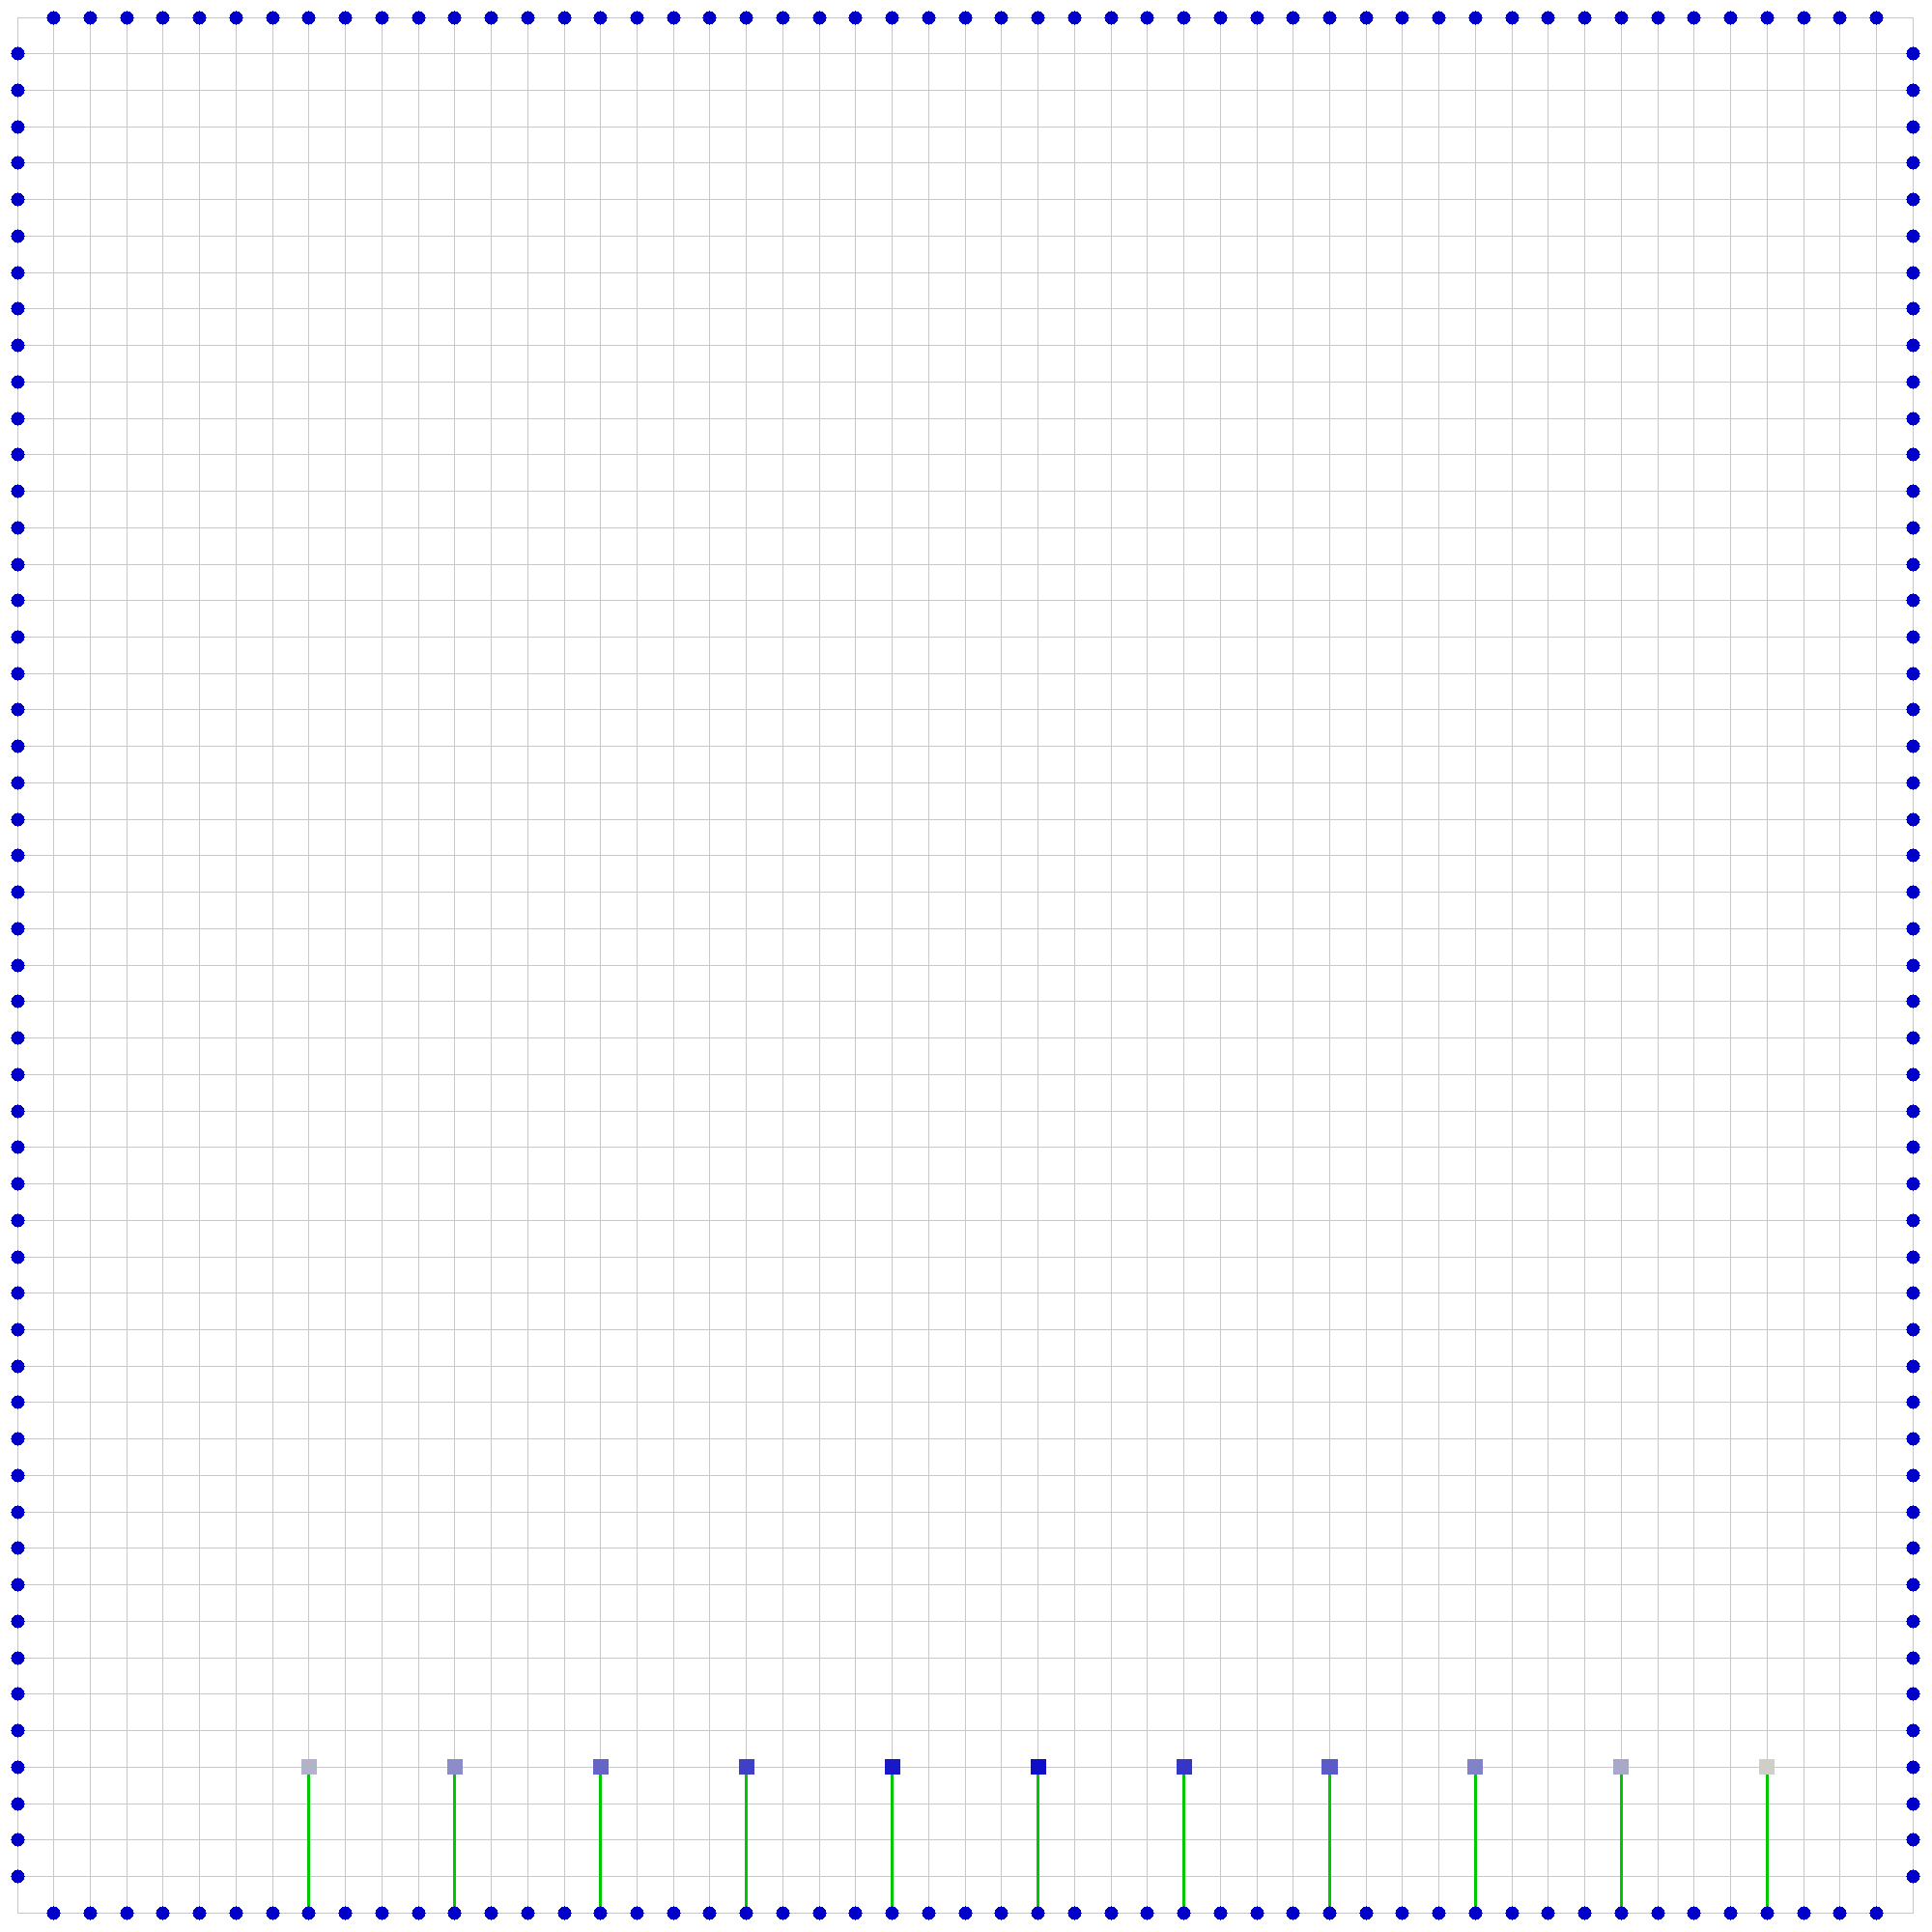
\includegraphics[width=2in]{12_1.png}
	\end{figure}
	\item 从最中间的部分,将三角形顶上的节点尽量连接出去。比如:
	\begin{figure}[H]
		\centering
		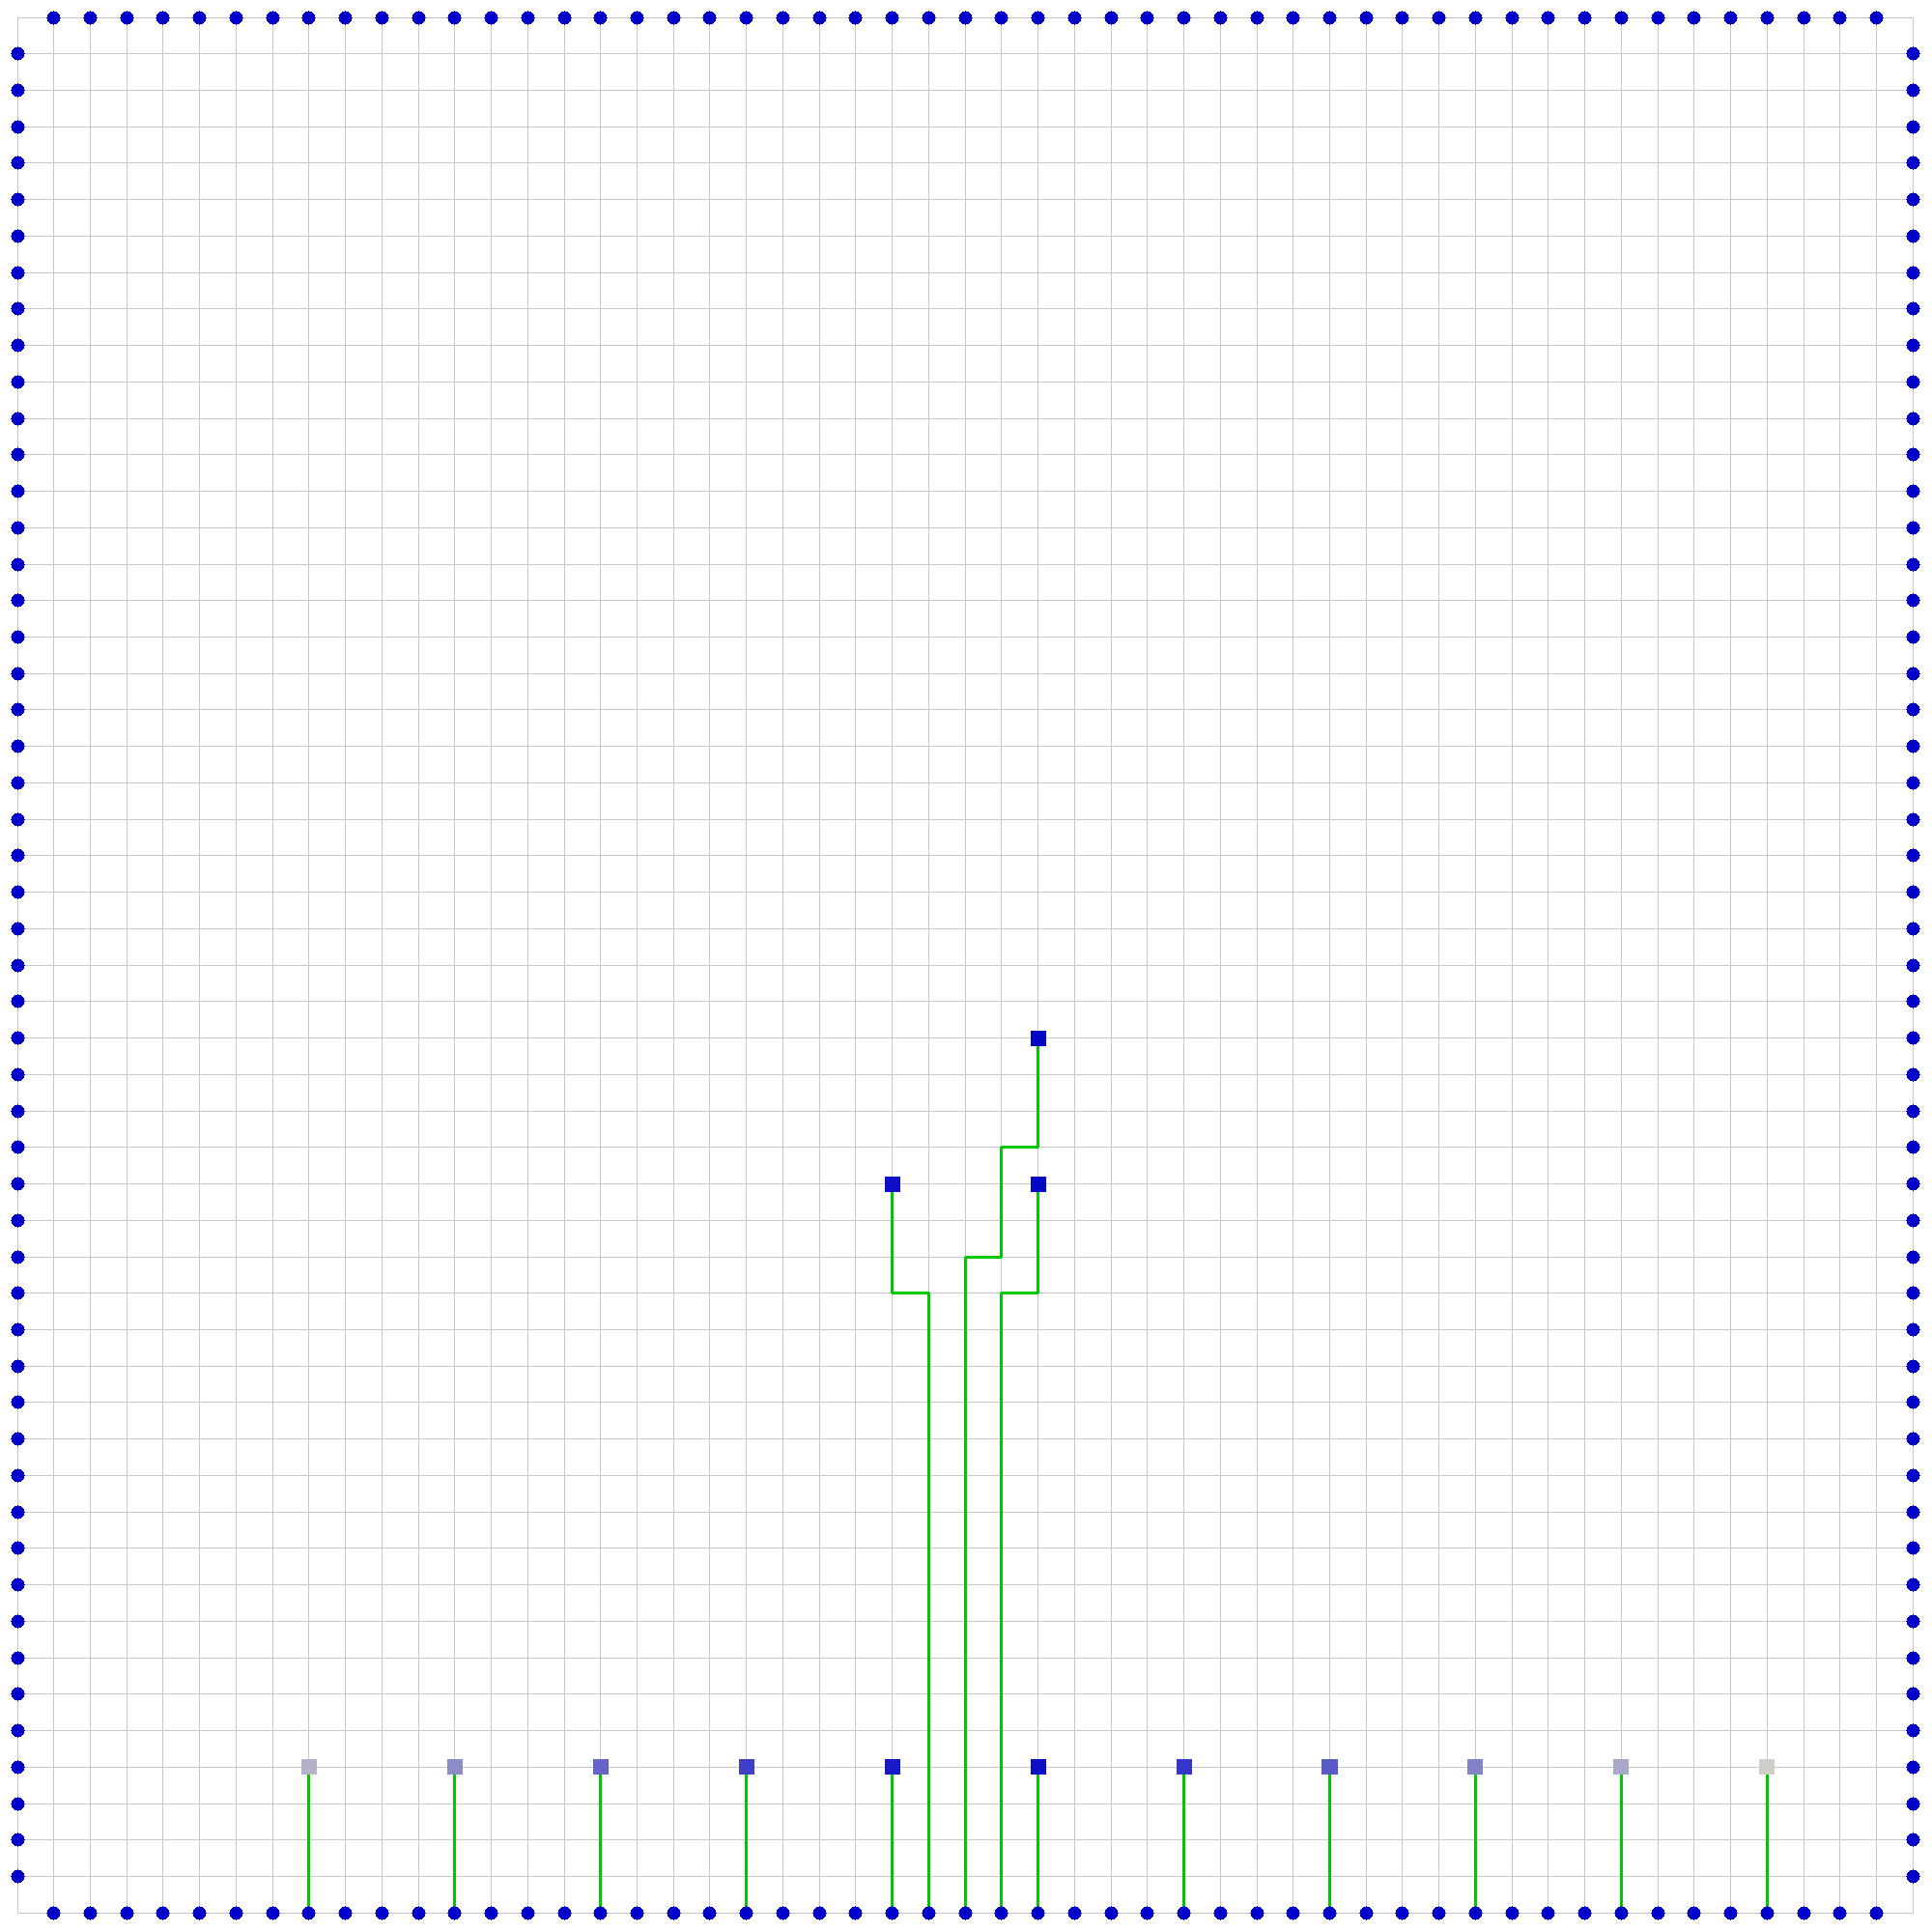
\includegraphics[width=2in]{12_2.png}
%		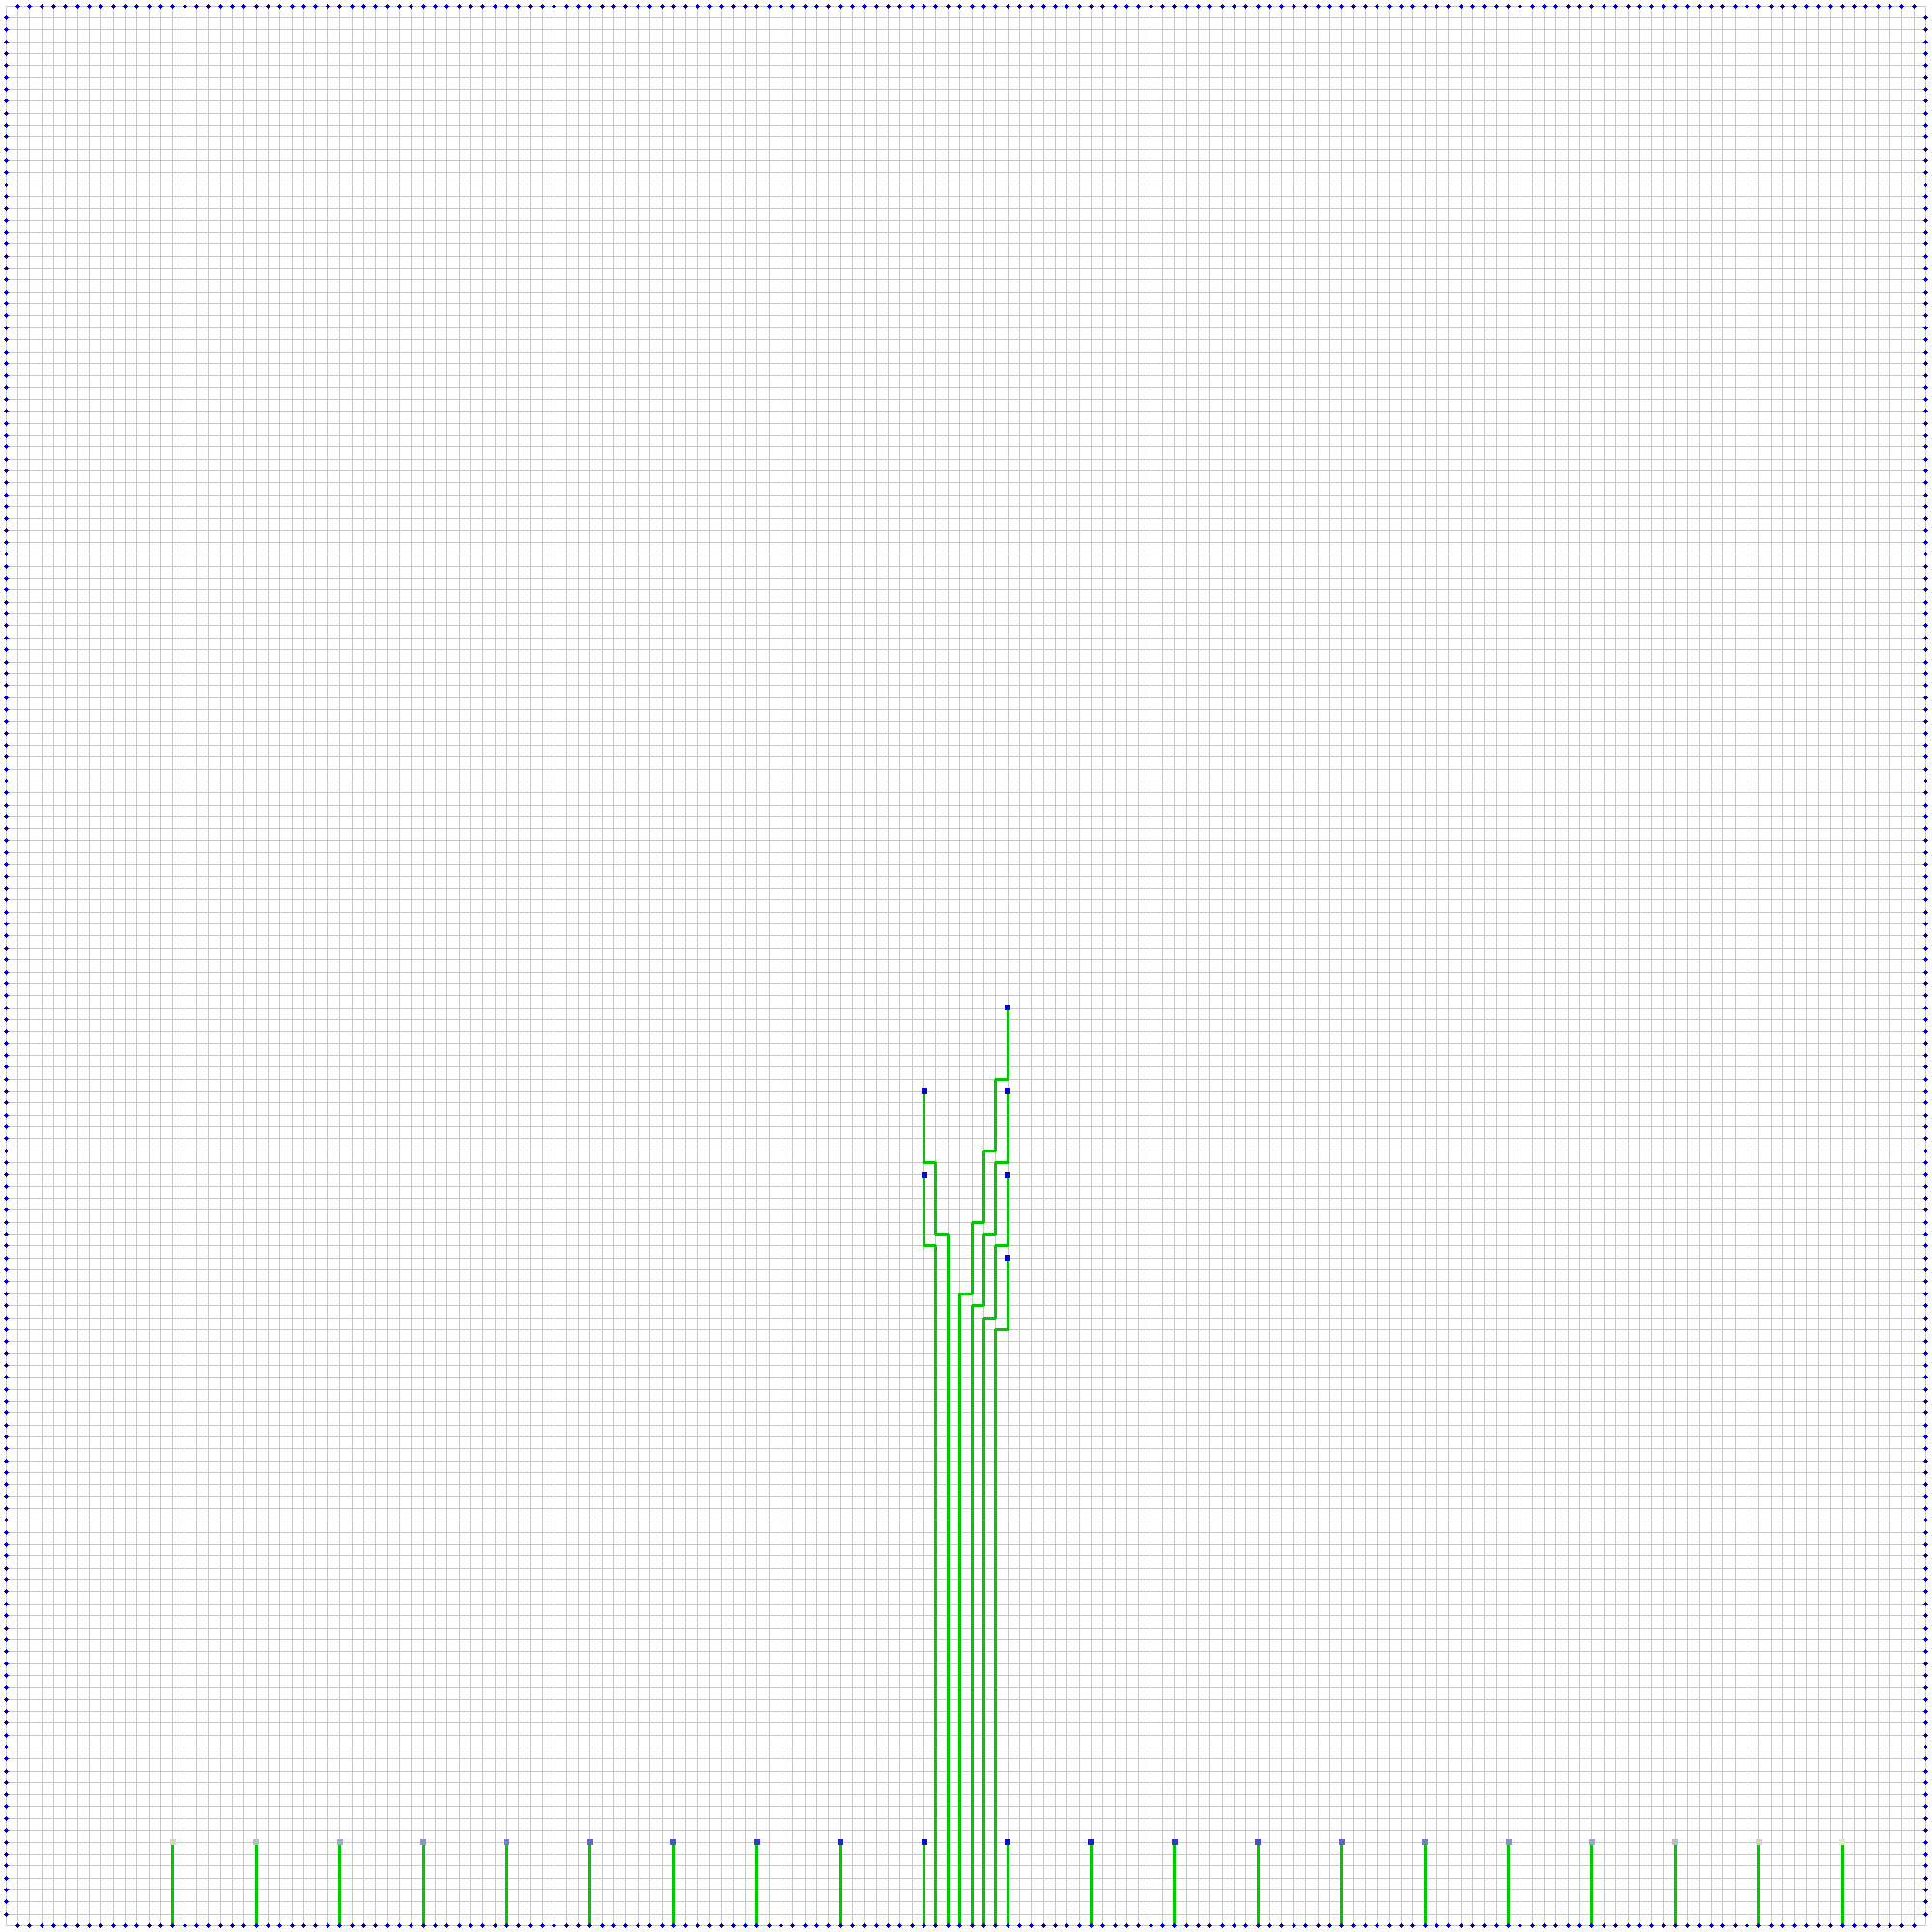
\includegraphics[width=2in]{22_2.png}
	\end{figure}
	\item 从中间向两边拓展。以左侧$\frac{1}{8}$的三角形为例,如果最右端还未被连接出去的点$A$可以执行连接操作,并且不会与其他尚未连接的点的连接发生冲突(即不存在某个点$B$,在$A$连接后,不存在任何一条路径,使得它能够被连接出去),那么就将$A$连接,并且出口尽量靠右。一个中间过程图如下图左图:
	\begin{figure}[H]
		\centering
		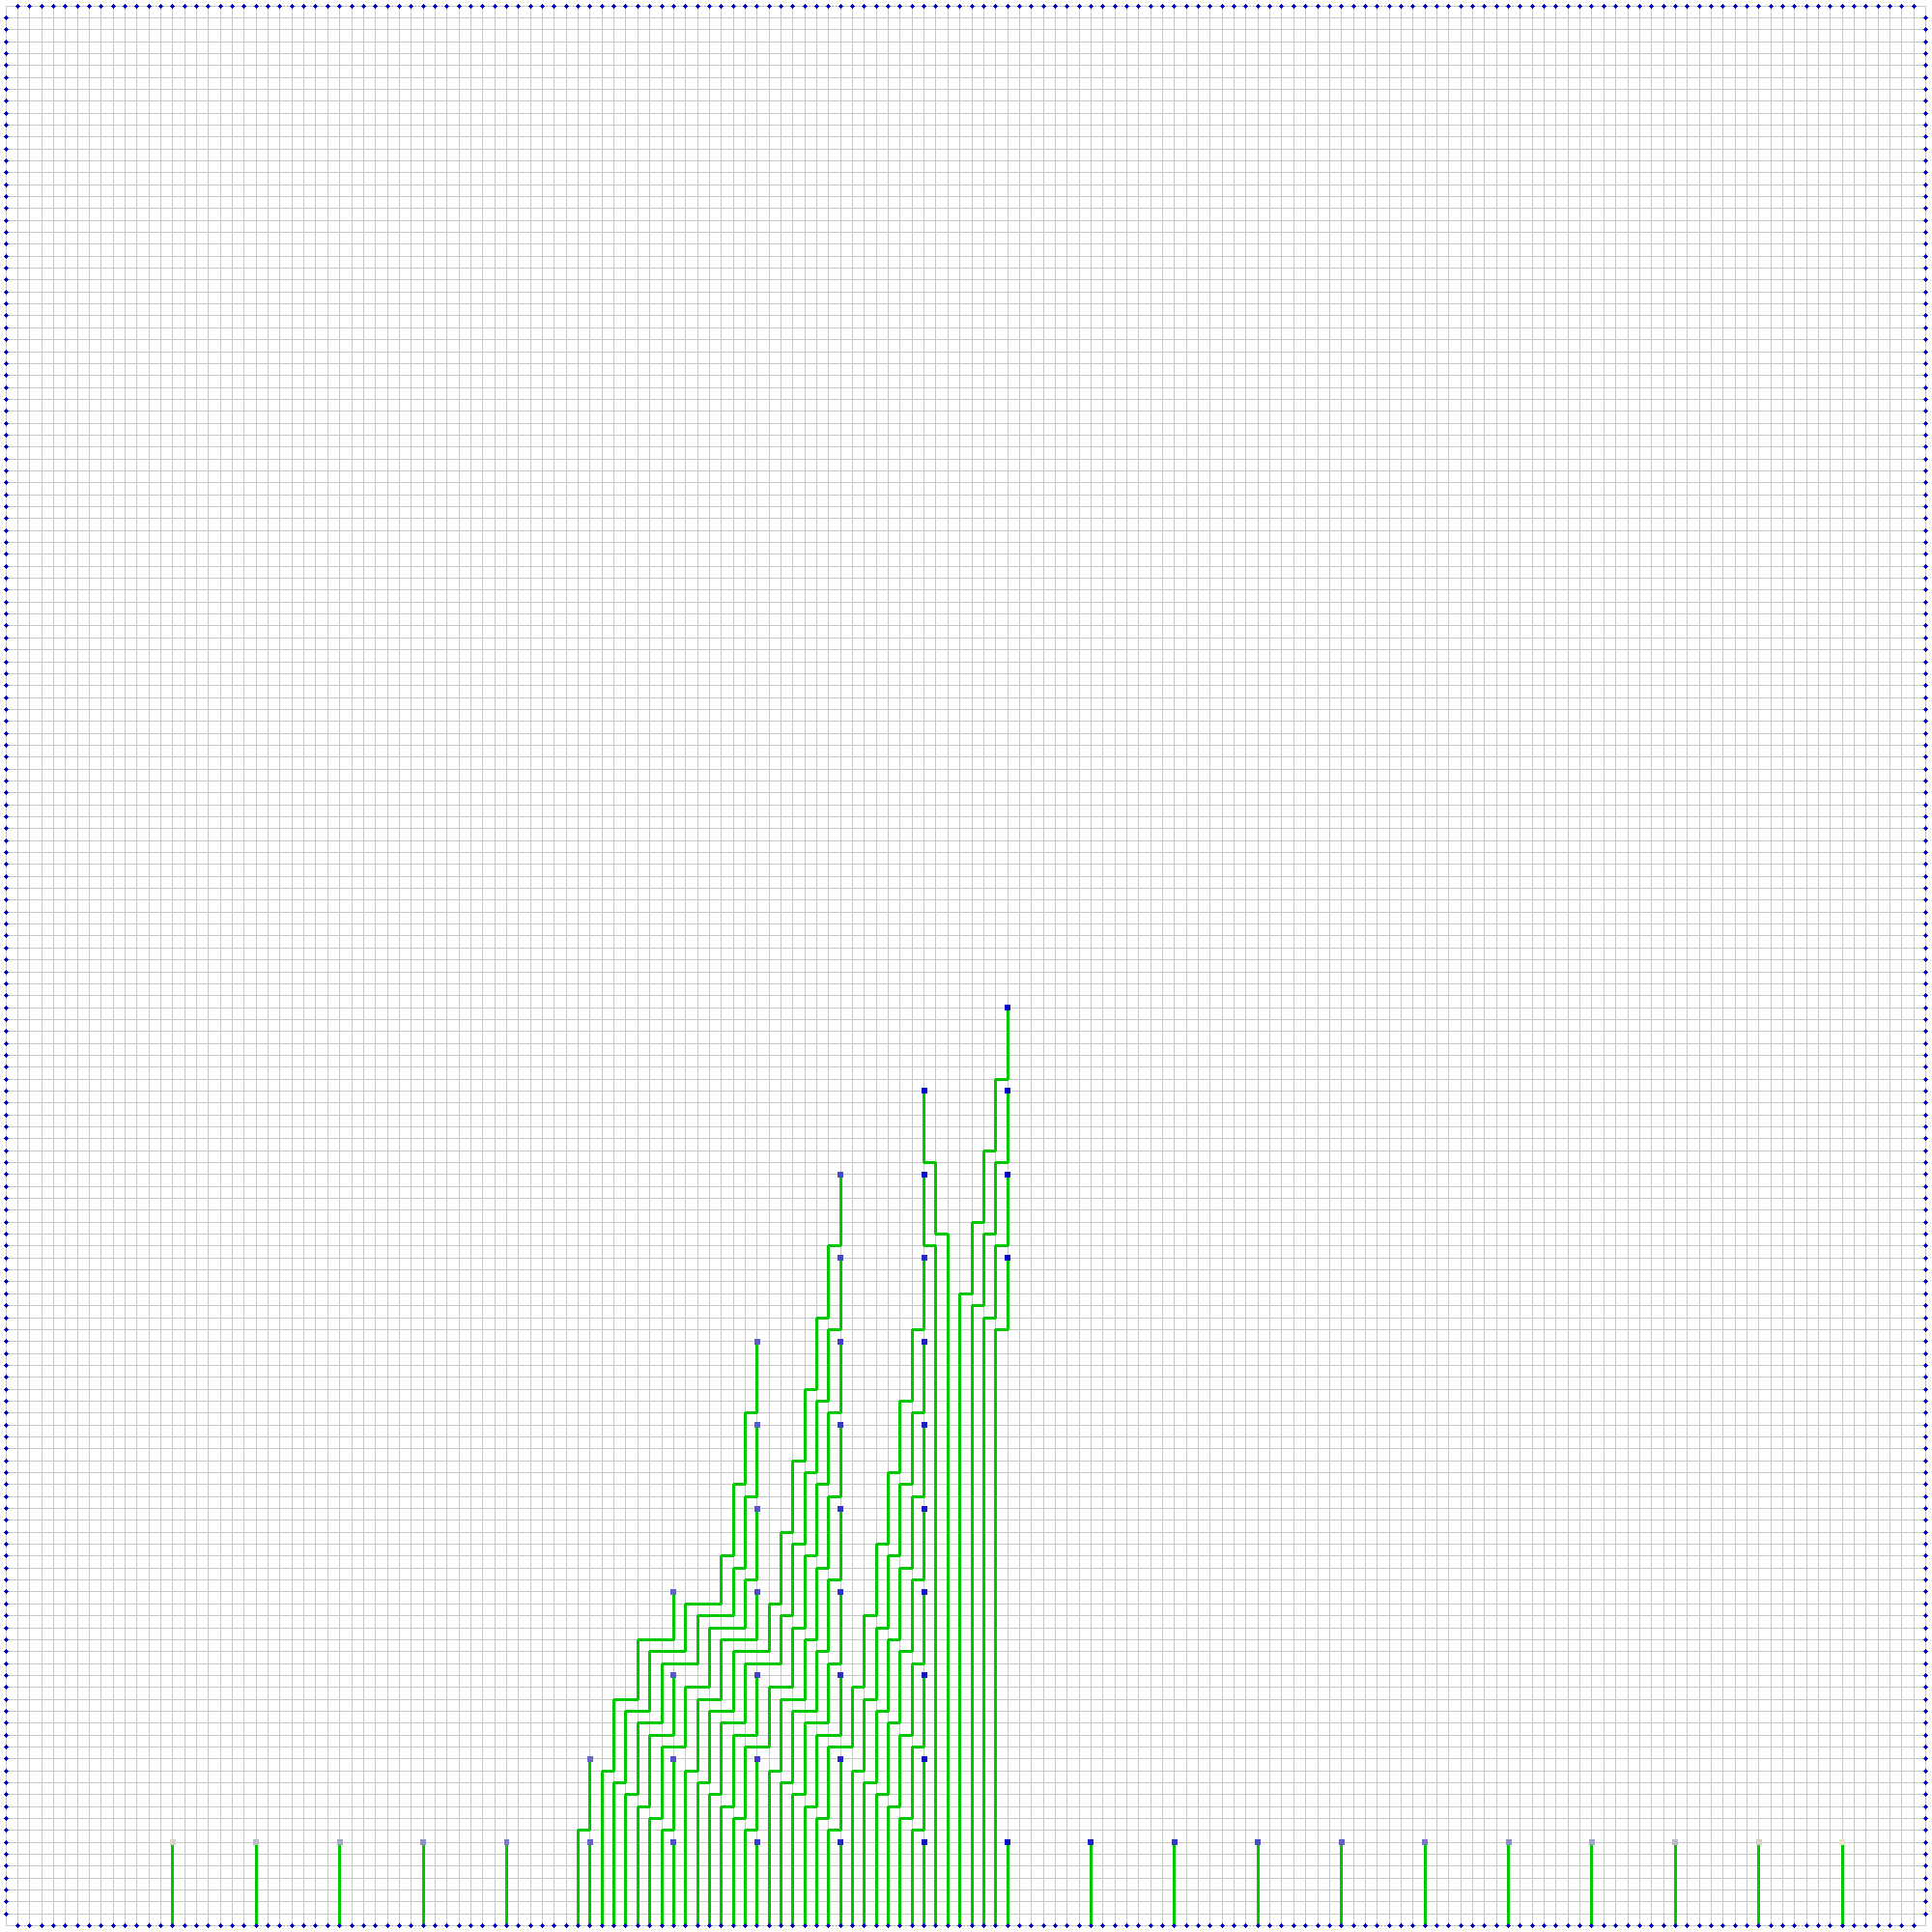
\includegraphics[width=2in]{22_3.png}
		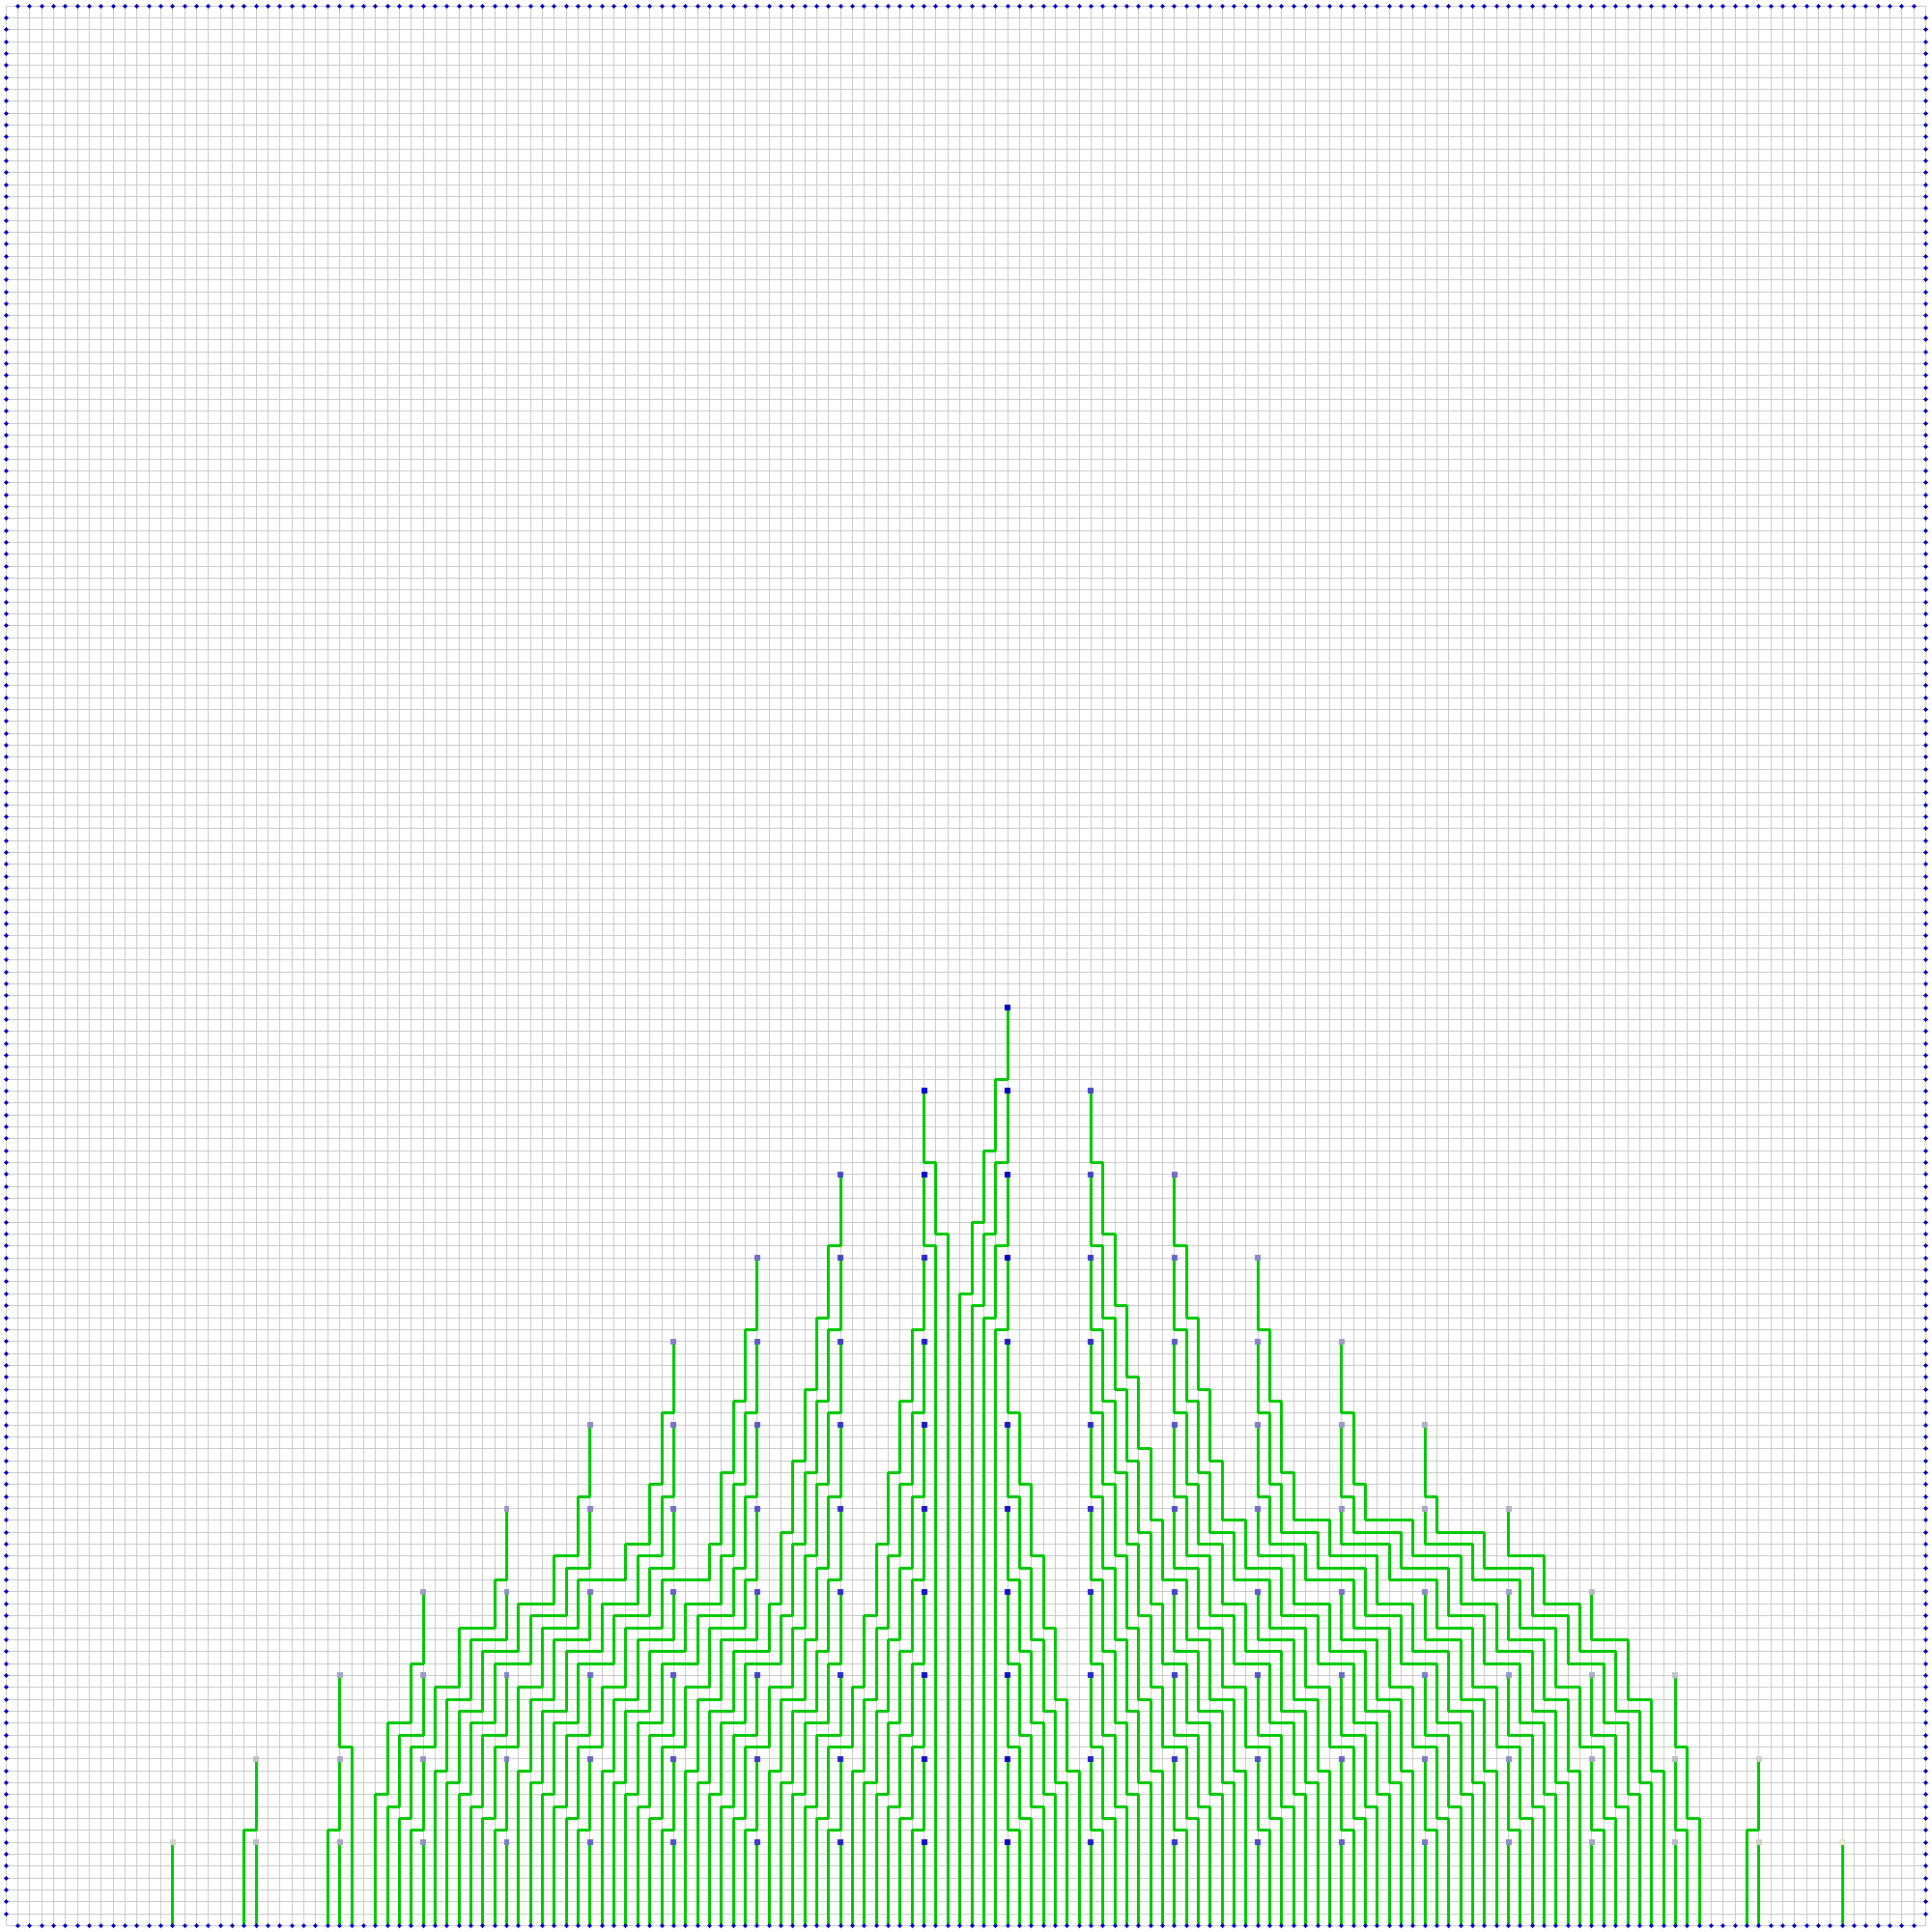
\includegraphics[width=2in]{22_4.png}
	\end{figure}	
	\item 处理两边角未被连接的节点。随便连一连就好了。最终这个$\frac{1}{4}$的三角形会变成上图右图那样。
	\item 最后将这四部的结果合并即可。
\end{enumerate}

在实现过程中,考虑到$80\times 80$的数据,网格图有$1945\times 1945$的大小,因此寻找路径的算法成为了效率实现的瓶颈。作者使用了$A^*$算法替代传统的BFS算法,估价函数设计成尽量贴着已存在的路径进行寻路,从而实现了效率正比于路径长度的高效算法。

经检验,该算法在$1\sim 80$的数据中只有两个数据需要一些微调,其他数据均快速出解,具体的效果详见下一章节。

\section{性能评测}

\subsection{运行性能测试}
\qquad
作者通过比对最小费用最大流算法\emph{MCMF}(能得出最优解)、\emph{Dinic}网络流算法(能得出可行解)、基于规则的布线算法\emph{Rule}(能得出次优解)的运行时间,来比较这三种方法的运行效率。

%我是把布线之后点与点的宽度估计成了logN
理论上分析,对于n个点,m条边并且容量都为1的\emph{MCMF},时间复杂度为$O(nm^2)$,而\emph{Dinic}的时间复杂度为$O(\min{(n^{2/3},m^{1/2})}\cdot m)$。在这个问题中,记$n^2$为需要连接的点的个数,$n\in [1,80]$,$N$为电路板的边长,结果表明$\frac{N - 1}{n + 1}\in [\frac{n}{4}, \frac{n}{3}]$,因此可以知道$N = \Theta(n^2)$。

因此复杂度可估计为\emph{MCMF}:$O(n^6)$,\emph{Dinic}:$O(n^3)$。

而人工设计的基于规则布线的方法几乎是正比于布线的总长度,因此时间复杂度为$O(n^2)$。

运行效率具体如下表所示:\footnote{运行环境:Intel(R) i5-5200U CPU 2.20GHz}

\begin{table}[H]
\label{tab:1}
\centering
\begin{tabular}{|c|c|c|c|}
\hline
\emph{n} & \emph{MCMF} & \emph{Dinic} & \emph{Rule}\\
\hline
5 & 0.040& 0.040& 0.040\\
\hline
15 & 0.308&0.056 & 0.040\\
\hline
25 & 7.504& 0.404& 0.064\\
\hline
35 &3'25'' & 2.276& 0.148\\
\hline
45 &24'4'' & 14.656& 0.272\\
\hline
55 &数小时 &66.584 & 0.484\\
\hline
65 &数小时 &7'13'' & 0.904\\
\hline
75 &约$8\sim 9h$&约$1h$  & 1.712\\
\hline
\end{tabular}
\caption{性能测试,时间若未注明则以秒计}
\end{table} 

可以看到,在实际运行中,费用流算法极其耗时,数据一旦超过40就很难在短时间内出结果;\emph{Dinic}算法在数据大的时候还是能在数分钟以内就出解的;规则布线方法效率最高,在不到数秒内就能出解。

\subsection{运行效果分析}

\begin{table}[H]
\label{tab:2}
\centering
\begin{tabular}{|c|c|c|c|c|c|}
\hline
\emph{n} & \emph{MCMF} & \emph{Dinic} & \emph{Rule} & $\frac{Rule-MCMF}{MCMF}\%$&$\frac{Dinic-MCMF}{MCMF}\%$\\
\hline
5 & 79 & 79 & 79 & 0.000&0.000 \\
\hline
15 & 3862&3910&3879&0.440&1.243 \\
\hline
25 & 27394	&   27566	 &  27460	&0.241& 0.628\\
\hline
35 &101775	&  102051	&  101920	&	0.142&0.271\\
\hline
45 & 273183	 & 273811	&  273433	&	0.092 &0.230\\
\hline
55 & 602856	 & 603975	&  603241	&0.064 &0.186\\
\hline
65 & 1167116	& 1168932	& 1167662	&	0.047&0.156\\
\hline
75 & 2057345	& 2060192	& 2058082	&	0.036&0.138\\
\hline
\end{tabular}
\caption{效果分析}
\end{table}

\qquad 从表\ref{tab:2}中可以看出,\emph{Dinic}算法所得出的解在数据范围大的时候,误差均小于$1\%$;相比之下,规则布线方法的结果总是要优于\emph{Dinic},并且相对最优解的误差在数据越大的时候越小,在数据大的时候,误差更是小于万分之五。可以说这是一个很优秀的方法。

\end{document}
